\def\year{2017}\relax
%File: formatting-instruction.tex
\documentclass[letterpaper]{article} %DO NOT CHANGE THIS
\usepackage{aaai17}  %Required
\usepackage{times}  %Required
\usepackage{helvet}  %Required
\usepackage{courier}  %Required
\usepackage{url}  %Required
\usepackage{graphicx}  %Required
\usepackage[ruled,vlined]{algorithm2e}
\usepackage{comment}
\usepackage{amssymb}
\usepackage{subcaption}
\frenchspacing  %Required
\setlength{\pdfpagewidth}{8.5in}  %Required
\setlength{\pdfpageheight}{11in}  %Required
%PDF Info Is Required:
  \pdfinfo{
/Title (Toward Supervised Reinforcement Learning with Partial States for Social HRI)
/Author (Emmanuel Senft)}
\setcounter{secnumdepth}{0}  
 \begin{document}
% The file aaai.sty is the style file for AAAI Press 
% proceedings, working notes, and technical reports.
%
\title{Toward Supervised Reinforcement Learning with Partial States for Social HRI}

\author{Emmanuel Senft \\
CRNS \\
Plymouth University \\
United Kingdom\\
\And S\'{e}verin Lemaignan\\
CRNS \\
Plymouth University \\
United Kingdom\\
\And Paul Baxter\\
L-CAS\\
University of Lincoln\\
United Kingdom\\
 \And Tony Belpaeme\\
 CRNS\\ Plymouth University (UK) \\ ID Lab -- imec \\ Ghent University (BE)}

\maketitle 

\begin{abstract}

    Social interacting is a complex task for which machine learning holds
    particular promise. However, as no sufficiently accurate simulator of human
    interactions exists today, the learning of social interaction strategies has
    to happen online in the real world. Actions executed by the robot impact on
    humans, and as such have to be carefully selected, making it impossible to
    rely on random exploration. Additionally, no clear reward function exists
    for social interactions. This implies that traditional approaches used for
    Reinforcement Learning cannot be directly applied for learning how to
    interact with the social world. As such we argue that robots will profit
    from human expertise and guidance to learn social interactions. And as the
    quantity of input a human can provide is limited, new methods have to be
    designed to use human input more efficiently. In this paper we describe a
    setup in which we combine a framework called Supervised Progressively
    Autonomous Robot Competencies (SPARC), which allows safer online learning
    with Reinforcement Learning, with the use partial states rather than full
    states to accelerate generalisation and obtain more quickly a usable action
    policy.

\end{abstract}
%===============================================================================

\section{Introduction}

Human-Robot Interaction (HRI) studies how people and robot can co-exist in
 society, and how they can interact socially in different environments and
 contexts. Robot are expected to behave appropriately regardless of the domain
 of interaction. However, it is impossible to foresee all possible interaction
 outcomes in dynamic and open social domains, as such the robot's responses
 cannot be implemented in the robot before its deployment in the real world.
 Similarly to  people, robots need to be able to learn how to complete tasks
 through creating and optimising action policies. This includes learning social
 norms and how to make sense of the social world.

For a robot, interacting in the real world often requires taking in a diverse
 and large range of sensory inputs, which results in a high-dimensional sensory
 space. The robot then is required to select actions based on its current state
 in sensor space. However, parts of the state can be irrelevant to the current
 goal, and as such should not be taken into account when selecting the current
 action. Often, only a limited number of features in the space are important. To
 interact efficiently, a robot has to learn to identify these salient features
 and associate them with appropriate actions.

In previous work~\cite{senft2015sparc,senft2017supervised}, we introduced the
Supervised Progressively Autonomous Robot Competencies (SPARC), a way to teach a
robot an action policy while interacting based on a human supervisor intervening
and correcting actions before they were executed by the robot. In this paper, we
propose to extend this approach to allow the supervisor to highlight features in
the environment relevant for the selected action. During the action selection
phase, the robot can compare these features, defined as partial states, with the
current state to select an action. The selected action is presented to the human
supervisor, who can either correct the action or approve it for execution.

%===============================================================================

\section{Background}
\subsection{Reinforcement Learning}

The main framework for an agent to learn how to interact in an environment while
interacting is Reinforcement Learning
(RL)~\cite{kober2013reinforcement,sutton1998reinforcement}. In RL, an agent
interacting in an environment receives numerical rewards in reaction to its
actions. The agent subsequently learns an action policy to maximise the expected
cummulative discounted reward.

In many cases where RL achieves success, the agent has access to a virtual
environment where the only real cost of exploring is computational effort: the
agent can interact as long as needed to gather enough information on the
environment and the result of its actions on the environment in order to find a
sufficiently optimal action policy. Using simulation RL can achieve impressive
results, as shown in RL learning to play Backgammon in the
90s~\cite{tesauro1995temporal} to the more recent success in mastering the game
of Go~\cite{silver2016mastering}. Even when a virtual environment is available,
but especially when it is not, human knowledge and effort is required during the
design of the algorithm or the learning phase before the learning can be
successful.

\subsection{Human impact on Reinforcement Learning}

Initial knowledge is often a crucial step to allow an algorithm to learn an
efficient action policy. This knowledge, originating from human expertise, can
be exploited in many ways. 

\subsubsection{Design decisions:}

Initial knowledge has to be used in the design of the algorithm, the
representation of the state and actions spaces and the reward funtion. For
example, only carefully crafted features allowed Tesauro to improve its
algorithm for Backgammon from a intermediate-level player to super-human
level~\cite{tesauro1995temporal}. Similarly, the design of complex neural
networks for state generalisation, the representation of actions as motor
primitives rather than raw motor angles or adding additional information in the
reward function have important impacts on the ability of the robot to reach a
successful policy~\cite{kober2013reinforcement}.

\subsubsection{Demonstrations:} 

Initial knowledge can be provided to the agent through demonstrations. These
demonstrations can be used to create an initial policy which is sufficiently
efficient to start interacting in the environment and gather information to
improve over time. This initial policy, required to receive meaningful feedback
from the environment can be impossible to reach by relying only on random
exploration and feedback from the environment. For example the game of Go in its
larger board size contains more than $10^{210}$ states, so exhaustive search is
not possible.  Silver et al.~\cite{silver2016mastering} started with supervised
learning from Go masters' games to learn a decent enough policy and then
proceeded using deep learning, self play and tree search to achieve super-human
capabilities and beating the best human players.

These demonstrations can also be used to learn a reward function. With Inverse
Reinforcement Learning, the agent is not provided with a reward function, but
derives it instead from a set of expert demonstrations. The agent can then
explore around the demonstrated policy to optimise the reward function. With
this approach, Abbeel and Ng achieved better than human control for a robotic
helicopter~\cite{abbeel2004apprenticeship} based on demonstrations from experts
and further exploration and autonomous learning.

\subsubsection{Guiding the learning:}

Rather than solely providing initial knowledge to the agents, humans can also
guide the agent during its learning, a method more resembling human teaching. 

A first approach consists in sequencing the tasks the robot will face.  This
approach, known as ``scaffolding''~\cite{saunders2006teaching}, progressively
increases the difficulty and complexity of the task as the robot is learning to
reach policies which would take prohibitively long without scaffolding.

Approaches from animal conditioning have also been transfered to Machine
Learning. For example, the TAMER framework~\cite{knox2009interactively} is an
adaptation of ``shaping'', tuning an animal's behaviour by providing rewards to
guide it to the desired behaviour. Unlike other RL setups, with TAMER, the
reward is not provided by the environment but by a human observer. With this
approach the teacher can adapt the rewards to the current policy and performance
of the agent, for example starting to positively reward suboptimal behaviours
that are better than the current policy and later, as the agent improves its
behaviour, reward these same suboptimal behaviours negatively and only the
optimal ones positively.

Another approach to guide the learning is to bias the action selection.
In~\cite{thomaz2008teachable}, the authors propose to use a human supervisor to
supply an agent with both rewards and potential guidance indicating what the
agent should pay attention to, or what action it should take next. They show
that giving the power to the supervisor to bias the action selection can improve
the learning, making it faster and safer.

In~\cite{senft2015sparc}, we introduced the Supervised Progressively Autonomous
Robot Competencies (SPARC). SPARC relies on a supervisor with the ability to
control the robot's actions. This supervisor is presented with the action the
robot is about to execute. He can then choose to cancel it, allow it to be
executed, or can select an alternative action. Based on the supervisor's
decisions, the robot learns which actions are desired and can as such refine its
policy over time reducing the need for the supervisor to correct or select an
action.

SPARC gives control of the robot's actions to an expert, who can guide the
exploration in the desired part of the environment which ensures the robot's
behaviour is consistently appropriate. As the exploration is guided, and all the
actions are useful, the learning can be faster than autonomous learning or
feedback based learning as illustrated in Figure~\ref{fig:comparison}.

\begin{figure}
    \centering
    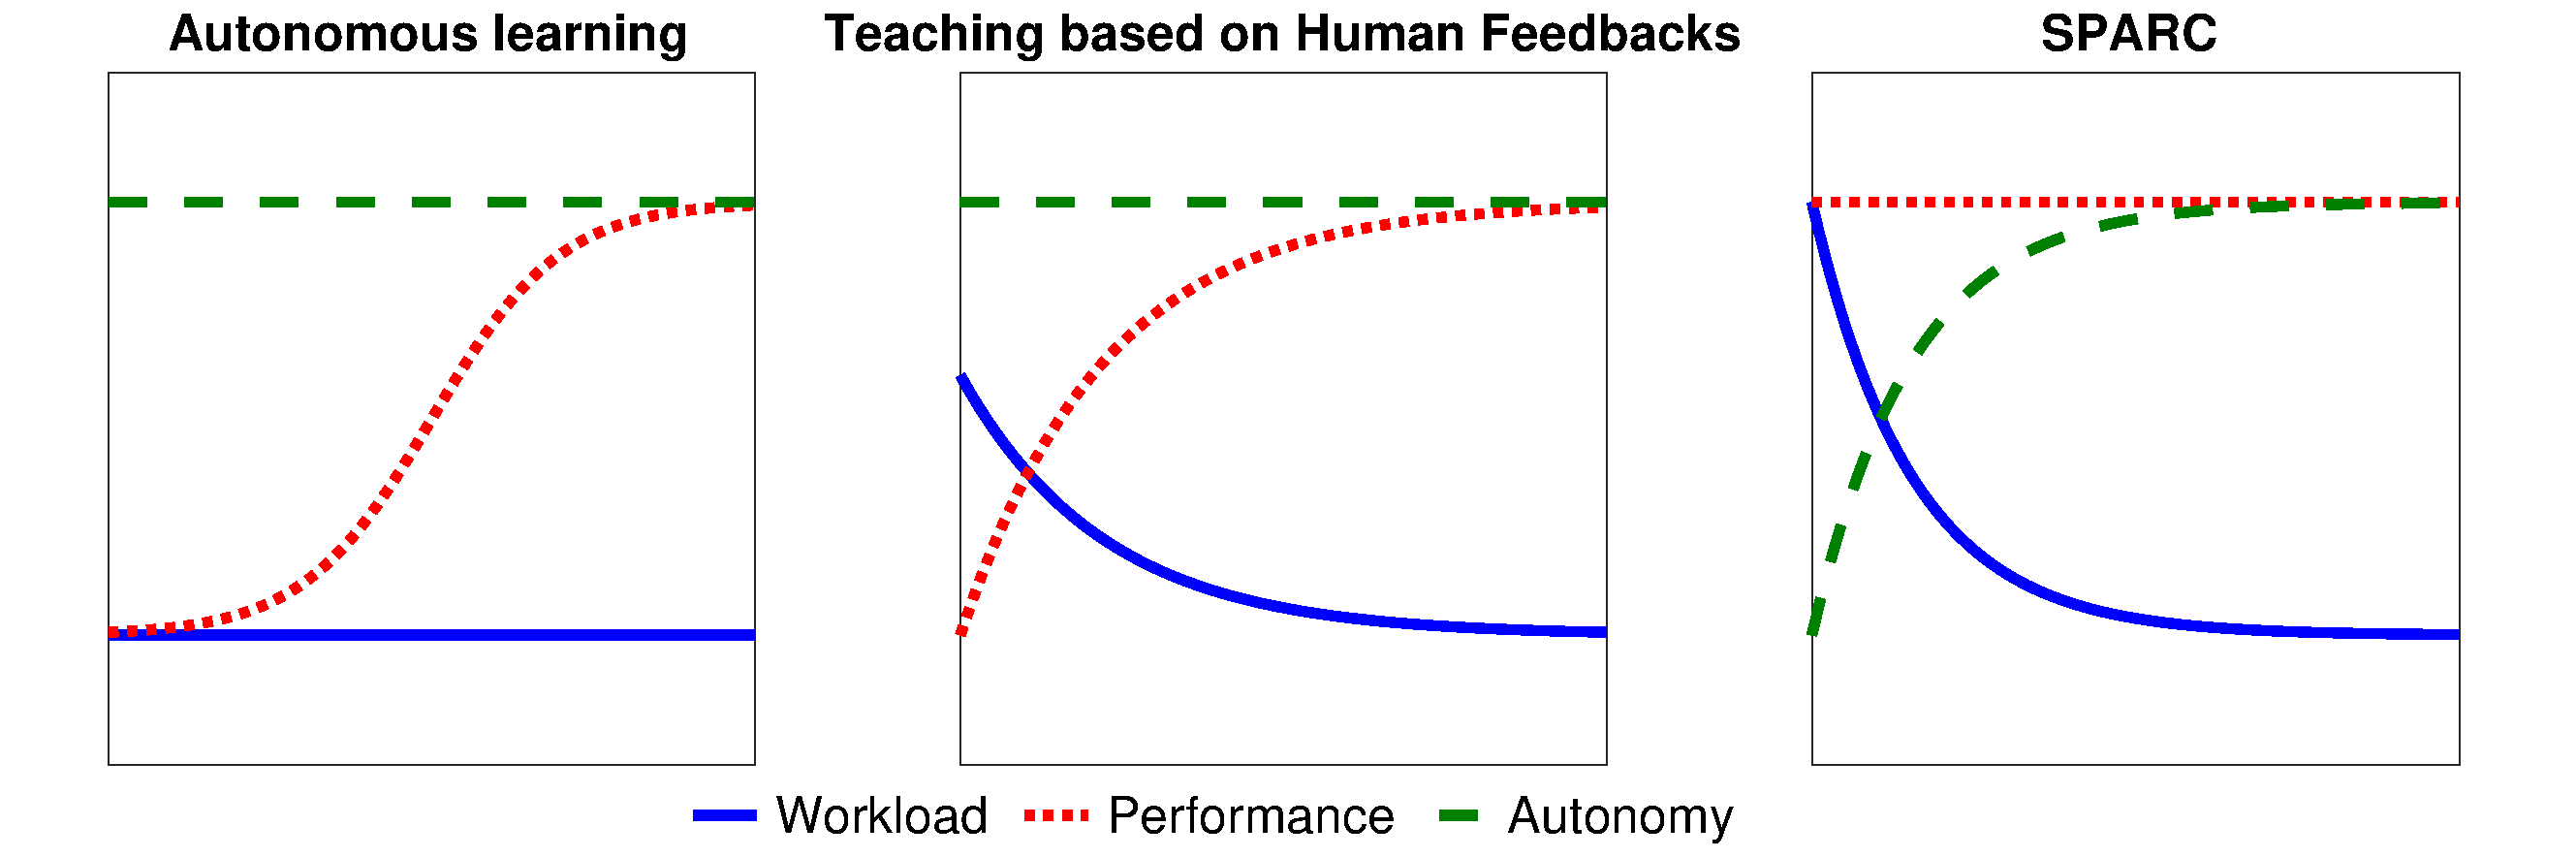
\includegraphics[width=0.9\linewidth]{./figs/motivation.pdf}
    \caption{An illustration of the evolution over time of the performance,
    autonomy and human workload for an autonomous learner, an approach using
    human rewards, and SPARC.}
    \label{fig:comparison}
\end{figure}

In~\cite{senft2017supervised}, we presented a way to combine SPARC and RL, by
assigning a positive reward to every action executed by the robot, making the
assumption that every action has been explicitly or implicitely approved by the
supervisor. However this method was directly mapping a single (state, action)
pair to a reward without making use of any kind of generalisation. As such it
was not applicable to environments with a continuous or high dimensional space
or non-deterministic transitions from one state to another, elements which are
typically present in social interactions.

\section{Partial State Supervised Reinforcement Learning}

To make RL applicable in high dimensional or continuous states, the algorithm
requires a way to generalise knowledge to unseen states. A classic approach is
to use a feed-forward neural network or to use deep reinforcement learning
relying on deep neural networks to learn a the value function. These approaches
rely on having a large number of datapoints to converge toward a good function
approximator. However, in many applications and especially in HRI, these amounts
of data are not available or obtainable due to practical constraints.
Furthermore, human responses are often noisy and lack consistency, so methods
are needed which can generalise from a low number of noisy data points.

In this paper we propose to use a human user to highlight the relevant features
of the environment to reduce the state dimension of the points only to relevant
information.  We introduce the concept of a partial state, a sliced version of
the state defined only on a subset of the dimensions of the state. This shifts
the (state, action) pair paradigm to (partial state, action)  and in the case of
RL, the tuple (state, action, reward) to (partial state, action, reward). This
allows to compare the current state and the datapoints only on relevant features
for action selection.

\subsection{Learning algorithm}

An expert supervises the agent actions, and can assign rewards to actions and
highlight the parts of the states which are relevant to assigning this reward to
this partial state.

As the supervisor can estimate the future impacts of an action, the problem of
credit assignment for delayed rewards can be ignored which allows us to consider
only a myopic approach. 

For this paper, we will reuse the formalism of rewardless Markov Decision
Process to identify the different elements of our system. The agent has access
to a set of actions $\mathcal{A}$ and a state $\mathcal{S} \in [0,1]^{n}$. We
also define the partial states $\mathcal{S'} \in [0,1]^{n'}$ with $n' \leq n$ as
a slice of $\mathcal{S}$, a subset of $\mathcal{S}$ where some dimensions have
been removed. 
%With each dimension of S representing features in the environment.

When the agent executes an action $a$ in state $s$, it receives the reward $r$
associated with the partial state $s'$. For example, a state $s$ could be
defined in 4 dimensions such as ${s=[1,0.2,0,0.5]}$, and $s'$ in two dimensions
with ${s'=[-,0.2,0,-]}$ with symbol '$-$' reprensenting the dimensions removed.
For the learning algorithm, this means that the action $a$ has been evaluated
$r$ in the partial state $s'$.  

To each action $a \in \mathcal{A}$ we can associate a set $\mathcal{C}_{a}$ of
pairs $(s',r)$ representing the rating done by the supervisor to action $a$ with
features highlighted for the multiple $s'$. When adding a new pair $(s',r)$, we
can discard potential previous pairs with an identical $s'$ to represent the
evolution of the policy evaluation by the supervisor.

\begin{algorithm}
    \DontPrintSemicolon
    \SetKwInOut{Input}{inputs}\SetKwInOut{Output}{output}
    \Input{Current state $s$, set of  $(a,s',r)$}
    \Output{selected action $\pi(s)$}
    \ForEach{$a \in \mathcal{A}$}{
        \ForEach{$p=(s',r) \in \mathcal{C}_{a}$}{
            compute similarity $\Delta$ between $s$ and $s'$:
            $\Delta(p)=1-\frac{\sum_{i}^{n'}(s'(i)-s(i))^{2}}{n'}$
        }
        compute expected reward $\hat{r}(a)$ for taking $a$ in $s$:
        $\hat{r}(a) = max(\Delta) \cdot r(arg\, max_{p} \Delta(p))$\\
        with $r(\Delta(p))$ the reward of $p = (s',r)$ 
    }
    Select the action with the maximum expected reward:
    $\pi(s) = arg\, max_{a} \hat{r}(a)$

    \caption{Algorithm for selecting an action based on the previous
    (partial state, action, reward) tuples and the current state.}
    \label{algo}
\end{algorithm}



When facing a new state $s$ where an action has to be selected, the agent can
select an action following Algorithm~\ref{algo}. For each action $a \in
\mathcal{A}$, we take the pair $(s',r)$ with the closest $s'$ to the current
state (as defined by normalised distance over the dimensions where $s'$ is
defined). That way, each action $a$ can be associated to an expected reward
defined by the product between the similarity of the closest partial state known
for $a$ and the reward obtained for executing $a$ in that partial state.
Finally, the action with the highest expected reward can be selected.

%When selecting an action, the agent can also use
%the dimensions of the close state $s'$ used for the selection to indicate the
%supervisor which parts of the state have been used for the action selection.

\subsection{Combination with SPARC}

SPARC has been shown to be compatible with RL in~\cite{senft2017supervised}, and
can also be easily combined with the approach presented in this paper using
partial states. For example, when selecting an action for the robot to be
executed, the supervisor can also select which features in the environment
should be selected as the partial state, and this associates the reward to this
action in this partial state. Similarly, when an action is proposed to the
supervisor the features represented by the dimensions of the closest partial
state for this action can be exposed to the supervisor as a way to explain why
this action has been selected. Facing this, the supervisor can: (1) not react,
allowing the action to be executed and associating a reward of +1 to the partial
state and the action proposed, (2) change the partial state to correct the
features related to this action or (3) cancel it, preventing the execution and
associating a reward of -1 to the partial state identified by the robot or the
supervisor. 

\section{Application scenario}


An example of an application is a social robot which interacts with children in
an educational scenario.  The robot plays an educational game with children to
teach them notions about diverse topics according to the needs of the teacher.
For this example, a child and a robot are playing a game about the food web,
teaching which animals eat which ones on a Sandtray~\cite{baxter2012touchscreen}.
In addition to the child and the robot, an adult supervises the robot using a
tablet with a Graphical User Interface (GUI) to teach the robot how to interact
with the child as shown in Figure~\ref{fig:setup}.

\begin{figure}
        \centering
  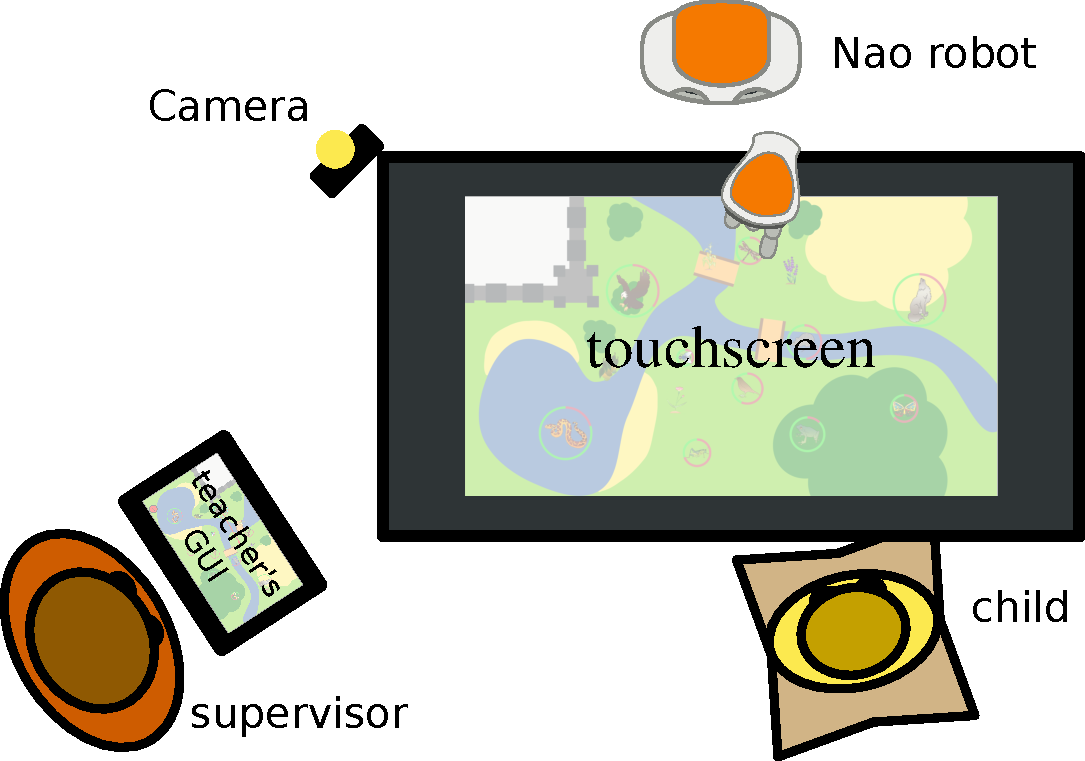
\includegraphics[width=60mm]{./figs/setup} 
    \caption{Interaction setup: the child and the robot are interacting on the
    touchscreen and a supervisor can control the robot using a GUI on a tablet.}
        \label{fig:setup}
\end{figure}


The GUI (Figure~\ref{fig:gui}) is an augmented version of the game itself, which
can be use to make the robot move items on the game by dragging them on the GUI
or which can display actions proposed by the robot with a cancel button to
refuse an action. For example in Figure~\ref{fig:gui} the robot proposes to move
the eagle to the rat, and highlight (as shown by blue circles) the eagle and the
rat. This indicate that features relevant to the eagle and the rat have been
used to select this action.

In the current implementation, the state is defined by the distance between each
animal and their energy. With these features selected, the partial state
transmitted to the user is the distance between the eagle and the rat, the
eagle's energy and
the rat's energy. Similarly, when selecting an action, the supervisor can 
select features in the state relevant to the action.

\begin{figure}
        \centering
    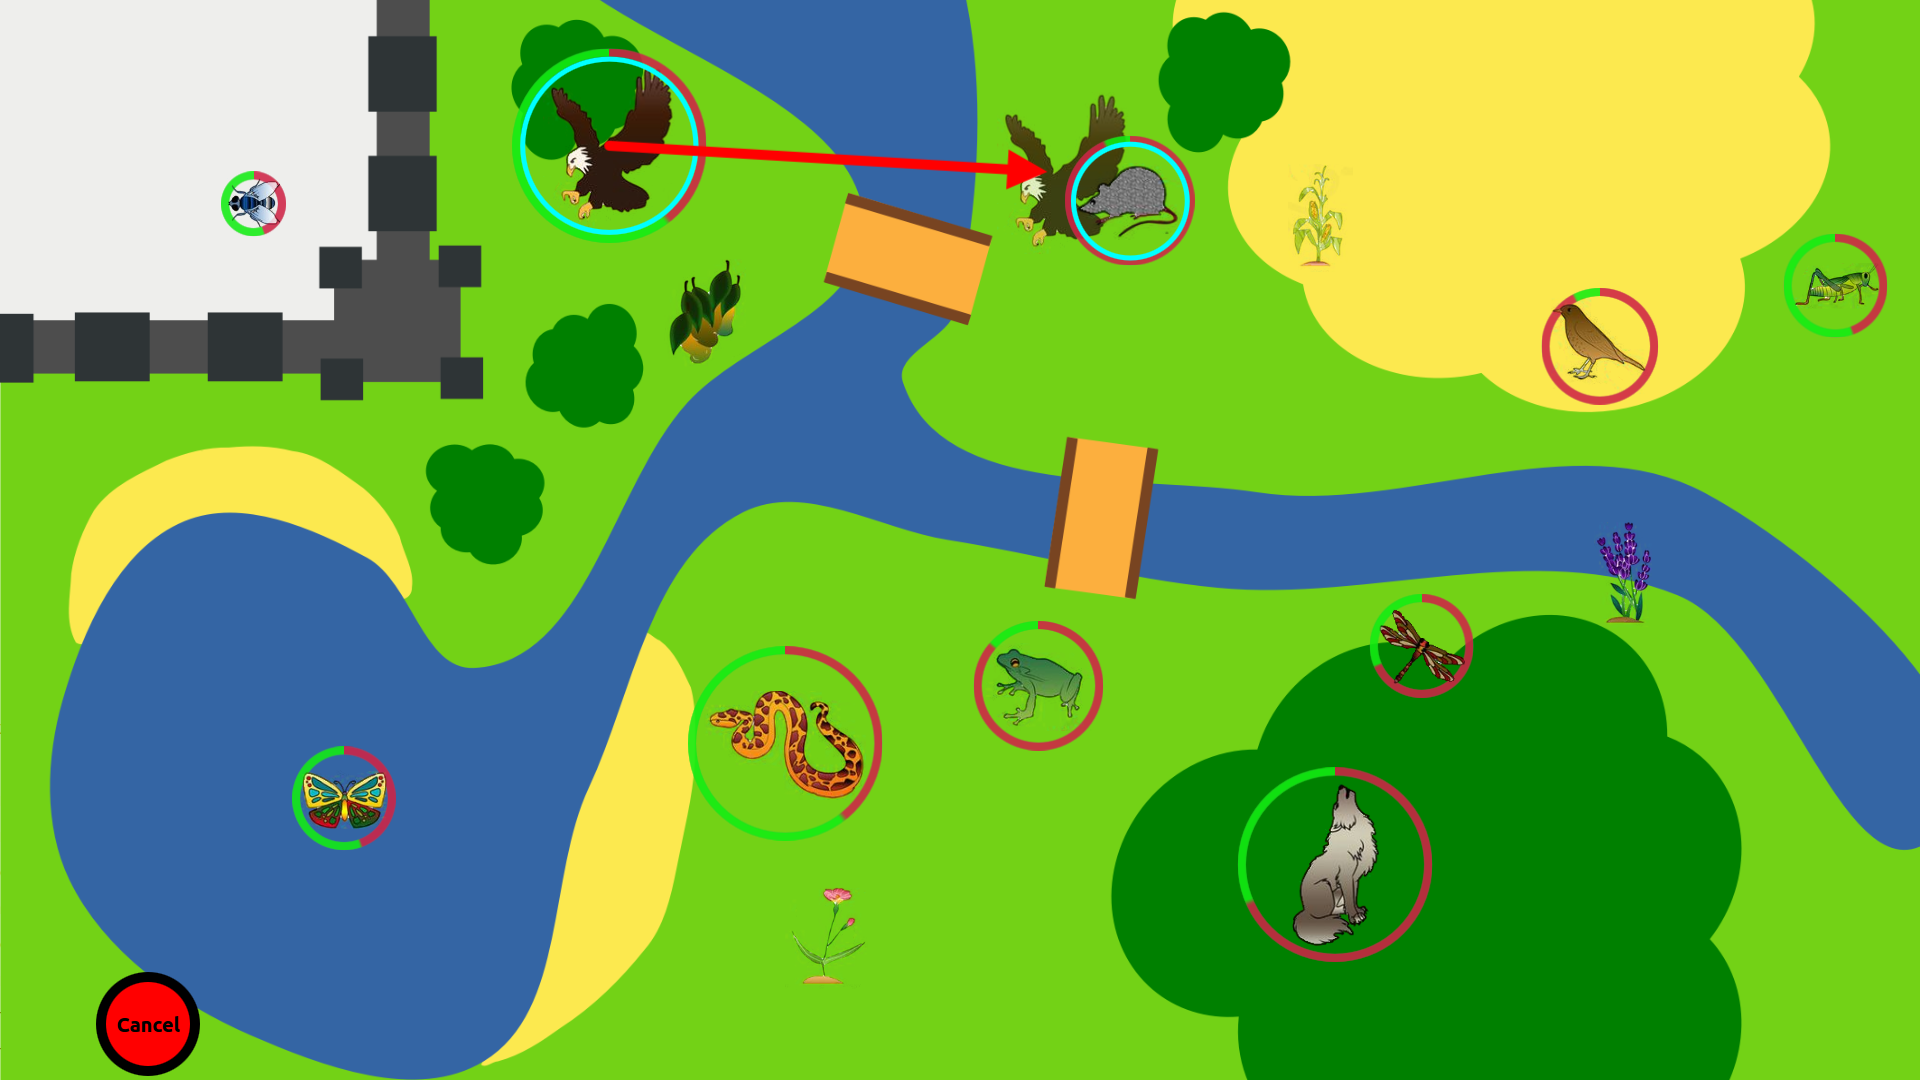
\includegraphics[width=60mm]{./figs/proposition.png}
    \caption{Interface for the supervisor with an action being proposed, moving
        the eagle to the rat with highlight of the eagle and the rat.}
        \label{fig:gui}
\end{figure}


The main limitations of the approach reside in the difference of
representation of the state and action spaces between the supervisor and the
algorithm and the limit in communication. For example a user could try to move
an animal close to another one,
and depending on the representation of the actions on the algorithm side, the
action might not be understood in the same way. Similarly, features used by the
supervisor to select actions might not be represented in the state used by the
algorithm. And lastly, in the case of implicit selection of features, a single
case of features representation (for example highlighting two animals) might not
be perceived in the same way by observers.


%===============================================================================
\section{Future work}

The system presented in the previous section will be improved and
evaluated in the real world with children in the next months.

The current work could also be extended to allow the agent to continue to
improve its behaviour even in the absence of a supervisor, progressively
exploring around the learnt policy improving its behaviour beyond the
demonstrations. This could be done by allowing the supervisor to provide rewards
during the learning phase and combine these rewards with the demonstrations to
learn a reward function in a fashion similar to Inverse Reinforcement
Learning~\cite{abbeel2004apprenticeship} or TAMER ~\cite{knox2009interactively}.
This could also use partial states associated to these rewards to ease the
generalisation of the reward function with only a low number of datapoints.  But
without the supervisor, the assumption that only a myopic action selection is
sufficient would not hold anymore and the problem of delayed rewards would have
to be tackled.

%==============================================================================
\section{Acknowledgments} This work was supported by the EU FP7 DREAM project
(grant no.  611391) and EU H2020 Marie Sklodowska-Curie Actions project DoRoThy
(grant 657227).  

\bibliographystyle{aaai} \bibliography{biblio}
\end{document}
